% Хавсралт A

%\chapter{Хавсралтын нэр} % Main appendix title

\label{AppendixA} % For referencing this appendix elsewhere, use \ref{AppendixA}
% \chapter*{Чухал кодын хэсгүүд}
% \section*{Хэрэглэгчийн бүртгэл үүсгэх кодын хэсэг}

% \begin{lstlisting}
% import numpy as np
    
% def incmatrix(genl1,genl2):
%     m = len(genl1)
%     n = len(genl2)
%     M = None #to become the incidence matrix
%     VT = np.zeros((n*m,1), int)  #dummy variable
    
%     #compute the bitwise xor matrix
%     M1 = bitxormatrix(genl1)
%     M2 = np.triu(bitxormatrix(genl2),1) 

%     for i in range(m-1):
%         for j in range(i+1, m):
%             [r,c] = np.where(M2 == M1[i,j])
%             for k in range(len(r)):
%                 VT[(i)*n + r[k]] = 1;
%                 VT[(i)*n + c[k]] = 1;
%                 VT[(j)*n + r[k]] = 1;
%                 VT[(j)*n + c[k]] = 1;
                
%                 if M is None:
%                     M = np.copy(VT)
%                 else:
%                     M = np.concatenate((M, VT), 1)
                
%                 VT = np.zeros((n*m,1), int)
    
%     return M
% \end{lstlisting}

\chapter*{Нэмэлт usecase тодорхойлолтууд}
\begin{longtable}{|r|p{11.5cm}|}
    \caption{Ажил олгогчоор бүртгүүлэх юзкейсийн тодорхойлолт}
    \label{table:usecase2}\\ \hline
    {Юзкейс:} & {Ажил олгогчоор бүртгүүлэх}\\ \hline
    {ID:} & {2}\\ \hline
    {Үүсгэсэн:} & {Ц. Анужин}\\ \hline
    {Үүсгэсэн огноо:} & {2025-03-21}\\ \hline
    {Үндсэн тоглогч:} & {Зочин}\\ \hline
    {Нэмэлт тоглогч:} & {Байхгүй}\\ \hline
    {Товч тайлбар:} & {Зочин системд ажил олгогчоор бүртгүүлнэ.}\\ \hline
    {Өмнөх нөхцөл:} & {Байхгүй}\\ \hline
    {Үндсэн урсгал:} & {\begin{enumerate}[nosep]
        \item Зочин ажил олгогчоор бүртгүүлэх үйлдлийг сонгоно.
        \item Байгууллага болон бүртгэлийн мэдээллээ оруулна.
        \item Систем мэдээллийг шалгаж ажил олгогчийн бүртгэл үүсгэнэ.
    \end{enumerate}}\\ \hline
    {Дараах нөхцөл:} & {\begin{enumerate}[nosep]
        \item Зочин системд ажил олгогчоор бүртгэгдсэн байна.
    \end{enumerate}}\\ \hline
    {Альтернатив урсгал:} & {Байхгүй}\\ \hline
\end{longtable}

\begin{longtable}{|r|p{11.5cm}|}
    \caption{Чатботтой харилцах юзкейсийн тодорхойлолт}
    \label{table:usecase7}\\ \hline
    {Юзкейс:} & {Чатботтой харилцах}\\ \hline
    {ID:} & {7}\\ \hline
    {Үүсгэсэн:} & {Ц. Анужин}\\ \hline
    {Үүсгэсэн огноо:} & {2025-03-21}\\ \hline
    {Үндсэн тоглогч:} & {Ажил горилогч}\\ \hline
    {Нэмэлт тоглогч:} & {Байхгүй}\\ \hline
    {Товч тайлбар:} & {Ажил горилогч AI чатботтой харьцан өөрт тохирсон ажлын байрны саналыг авна.}\\ \hline
    {Өмнөх нөхцөл:} & {\begin{enumerate}[nosep]
        \item Ажил горилогч системд нэвтэрсэн байна.
    \end{enumerate}}\\ \hline
    {Үндсэн урсгал:} & {\begin{enumerate}[nosep]
        \item Ажил горилогч чатботын хуудас руу орно.
        \item Ажил горилогч өөрийн хүссэн цалин, байршил, чиглэлийн талаар мэдээлэл оруулна.
        \item AI хэрэглэгчийн хүсэлтийг боловсруулна.
        \item Систем тохирох ажлын байруудыг санал болгоно.
        \item Ажил горилогч санал болгосон ажлын байруудтай танилцана.
        \item Ажил горилогч нэмэлт асуулт тавих эсвэл харилцааг үргэлжлүүлж болно.
    \end{enumerate}}\\ \hline
    {Дараах нөхцөл:} & {\begin{enumerate}[nosep]
        \item Ажил горилогч өөрт тохирсон ажлын байрны мэдээллийг авсан байна.
    \end{enumerate}}\\ \hline
    {Альтернатив урсгал:} & {Байхгүй}\\ \hline
\end{longtable}

\begin{longtable}{|r|p{11.5cm}|}
    \caption{Ирсэн анкетуудыг харах юзкейсийн тодорхойлолт}
    \label{table:usecase9}\\ \hline
    {Юзкейс:} & {Ирсэн анкетуудыг харах}\\ \hline
    {ID:} & {9}\\ \hline
    {Үүсгэсэн:} & {Ц. Анужин}\\ \hline
    {Үүсгэсэн огноо:} & {2025-03-21}\\ \hline
    {Үндсэн тоглогч:} & {Ажил олгогч}\\ \hline
    {Нэмэлт тоглогч:} & {Байхгүй}\\ \hline
    {Товч тайлбар:} & {Ажил олгогч тухайн ажлын байранд ирсэн анкетуудыг AI үнэлгээний дүнтэй хамт харж шүүнэ.}\\ \hline
    {Өмнөх нөхцөл:} & {\begin{enumerate}[nosep]
        \item Ажил олгогч системд нэвтэрсэн байна.
        \item Тухайн ажлын байранд анкет ирсэн байна.
    \end{enumerate}}\\ \hline
    {Үндсэн урсгал:} & {\begin{enumerate}[nosep]
        \item Ажил олгогч ажлын зарыг сонгоно.
        \item Систем ирсэн анкетуудын жагсаалтыг тохирох хувиар эрэмбэлж харуулна.
        \item Ажил олгогч анкет бүрийн дэлгэрэнгүй үнэлгээг харна.
        \item Ажил олгогч шаардлагатай бол нэмэлт шүүлт хийнэ.
    \end{enumerate}}\\ \hline
    {Дараах нөхцөл:} & {\begin{enumerate}[nosep]
        \item Ажил олгогч анкетуудтай танилцаж дараагийн шатны шийдвэр гаргахад бэлэн байна.
    \end{enumerate}}\\ \hline
    {Альтернатив урсгал:} & {Байхгүй}\\ \hline
\end{longtable}

\begin{longtable}{|r|p{11.5cm}|}
    \caption{Даалгаврын гүйцэтгэлийг харах, үнэлэх юзкейсийн тодорхойлолт}
    \label{table:usecase12}\\ \hline
    {Юзкейс:} & {Даалгаврын гүйцэтгэлийг харах, үнэлэх}\\ \hline
    {ID:} & {12}\\ \hline
    {Үүсгэсэн:} & {Ц. Анужин}\\ \hline
    {Үүсгэсэн огноо:} & {2025-03-21}\\ \hline
    {Үндсэн тоглогч:} & {Ажил олгогч}\\ \hline
    {Нэмэлт тоглогч:} & {Байхгүй}\\ \hline
    {Товч тайлбар:} & {Ажил олгогч ажил горилогчийн илгээсэн даалгаврын гүйцэтгэлийг харж үнэлгээ өгнө.}\\ \hline
    {Өмнөх нөхцөл:} & {\begin{enumerate}[nosep]
        \item Ажил олгогч системд нэвтэрсэн байна.
        \item Ажил горилогч даалгаврыг гүйцэтгэж илгээсэн байна.
    \end{enumerate}}\\ \hline
    {Үндсэн урсгал:} & {\begin{enumerate}[nosep]
        \item Ажил олгогч даалгаврын жагсаалт руу орно.
        \item Систем илгээгдсэн даалгаврын гүйцэтгэлүүдийг харуулна.
        \item Ажил олгогч тухайн ажил горилогчийн гүйцэтгэлийг нээнэ.
        \item Гүйцэтгэлийг үзэж үнэлгээ өгнө.
        \item "Хадгалах" товчийг дарна.
        \item Систем үнэлгээг хадгалж ажил горилогчид мэдэгдэл илгээнэ.
    \end{enumerate}}\\ \hline
    {Дараах нөхцөл:} & {\begin{enumerate}[nosep]
        \item Үнэлгээ системд хадгалагдсан байна.
        \item Ажил горилогч үнэлгээний мэдэгдэл хүлээн авсан байна.
    \end{enumerate}}\\ \hline
    {Альтернатив урсгал:} & {Байхгүй}\\ \hline
\end{longtable}



% \chapter*{Нэмэлт шинжилгээний дарааллын диаграмм}
% \begin{figure}[H]
%     \centering
%     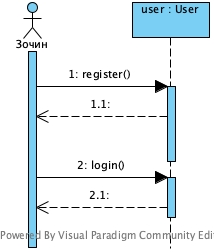
\includegraphics[scale=0.6]{Figures/chapter2/register.jpg}
%     \caption{Бүртгэл үүсгэх шинжилгээний дарааллын диаграмм}
%     \label{fig:burtgel-zh-1}
% \end{figure}